\documentclass[12pt, a4paper, answers]{exam} % Lösungen
%\documentclass[12pt, addpoints, a4paper]{exam} % Ohne Lösungen
\newcommand{\myAuthor}{Constantin Lazari, Marco Wettstein}
\newcommand{\myTitle}{Übungen Informatik}
\newcommand{\mySubject}{Informatik III (2013)}
\newcommand{\myNumber}{3}

\usepackage[utf8]{inputenc}
\usepackage[pdftex]{graphicx} 
\usepackage{microtype}
\usepackage[pdfborder={0 0 0}, plainpages=false, pdfpagelabels]{hyperref} 
\usepackage[ngerman]{babel}
\usepackage[babel]{csquotes}
\usepackage{tabularx} 

\usepackage{tikz}
\usetikzlibrary{arrows,automata}
\usepackage{amsmath,amssymb,amsthm}

\usepackage{lmodern} %Type1-Schriftart fuer nicht-englische Texte
\hyphenation{eine einer eines} % Trennung von eine, einer, eines vermeiden
\usepackage{microtype}

\usepackage{color}
\usepackage{stmaryrd}
\usepackage{booktabs}


%% Listings %%%%%%%%%%%%%%%%%%%%%%%%%%%%%%%%%%%%%%%%%%%%%%%%%
%\usepackage{verbatim}
\usepackage{listings}
\lstloadlanguages{[LaTeX]TeX}
{\lstset{%
  basicstyle=\footnotesize\ttfamily,
  commentstyle=\slshape\color{green!50!black},
  keywordstyle=\bfseries\color{blue!50!black},
  identifierstyle=\color{blue},
  stringstyle=\color{orange},
  escapechar=\#,
  emphstyle=\color{red}}
}
{
  \lstset{%
    basicstyle=\ttfamily,
    keywordstyle=\bfseries,
    commentstyle=\itshape,
    escapechar=\#,
    emphstyle=\bfseries\color{red}
  }
}

\hypersetup{
	pdfauthor   = {\myAuthor},
	pdftitle    = {\myTitle},
	pdfsubject  = {\mySubject},
	pdfkeywords = {},
	pdfcreator  = {Kile},
	pdfproducer = {pdflatex},
	colorlinks 	= false
} 

\setlength{\parindent}{0em}
\setlength{\parskip}{0.75em}

%% Exam Settings
\pagestyle{headandfoot}
%\firstpageheader{Benutzer/innen im Umgang mit Informatikmitteln instruieren}{}{Lernkontrolle 1}
\firstpageheader{\mySubject}{}{Übung \myNumber}
\firstpageheadrule

%\runningheader{Benutzer/innen im Umgang mit Informatikmitteln instruieren}{}{Lernkontrolle 1}
\runningheader{\mySubject}{}{
\ifprintanswers
  Lösung Übung \myNumber
\else
  Übung \myNumber
\fi
}
\runningheadrule

\firstpagefooter{}{Seite \thepage\ von \numpages}{}
\firstpagefootrule

\runningfooter{}{Seite \thepage\ von \numpages}{}
\runningfootrule

\pointsinrightmargin
\pointpoints{Punkt}{Punkte}
\bonuspointpoints{Bonuspunkt}{Bonuspunkte}
\renewcommand{\solutiontitle}{\noindent\textbf{Lösung:}\par\noindent}

\CorrectChoiceEmphasis{\bfseries}
\renewcommand\choicelabel{$\boxempty$}

\begin{document}
	\begin{tabularx}{\textwidth}{Xr}
	\myAuthor & \today\\
	\end{tabularx}
  %% Lernkontrolle einbinden
	\begin{questions}
	\question
Kontrollstrukturen, wie z. B. Schleifen in höheren Programmiersprachen, werden in Maschinensprache über Sprungbefehle realisiert.
\begin{parts}
\part
Skizzieren Sie graphisch (schematisch), wie eine For- und eine While-Schleife, die 10-mal ($n \geq 0$) durchlaufen wird, umgesetzt werden könnte.
\begin{solutionordottedlines}[2cm]
1. For-Schleife
\begin{center}
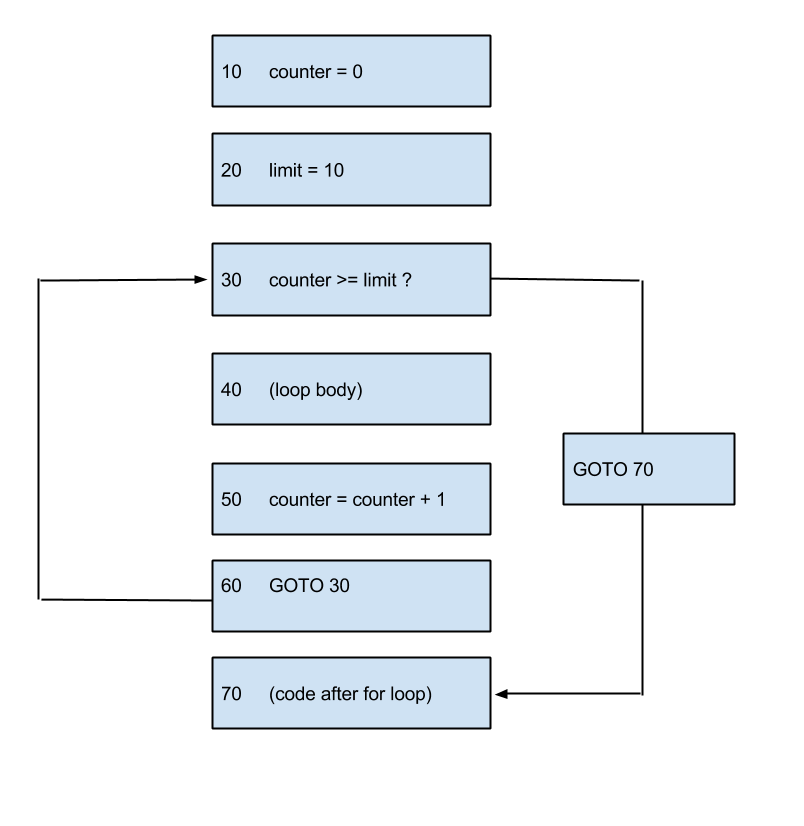
\includegraphics[width=\linewidth]{for-loop.png}
\end{center}
\pagebreak
2. While-Schleife
\begin{center}
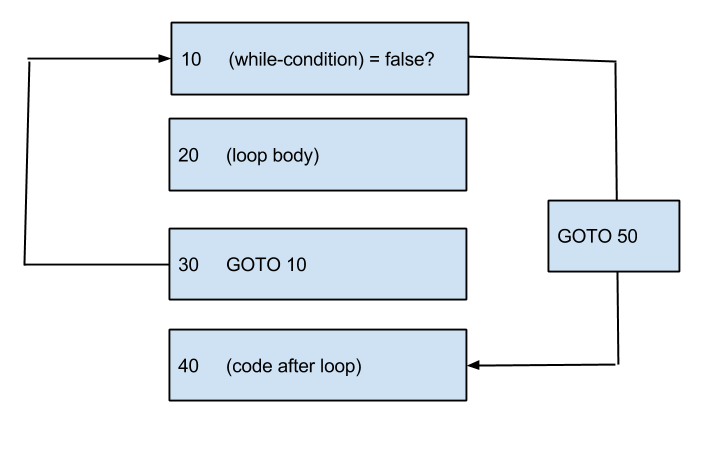
\includegraphics[width=\linewidth]{while-loop.png}
\end{center}
\end{solutionordottedlines}
%%% Next subquestion

\part
Mit welcher Einschränkung ist es möglich, die FOR-Schleife mit nur einem Sprungbefehl zu realisieren? Skizzieren Sie auch diesen Fall.
\begin{solutionordottedlines}[2cm]
\begin{center}
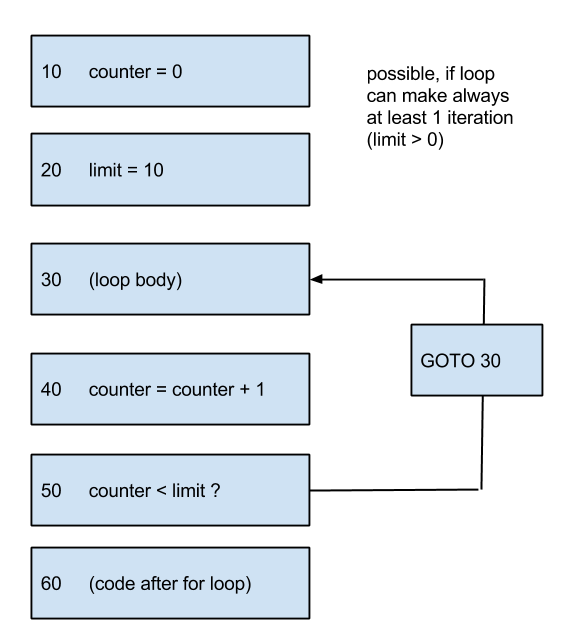
\includegraphics[width=0.7\linewidth]{for-loop-one-jump.png}
\end{center}
\end{solutionordottedlines}
%%% Next subquestion

\end{parts}
	\pagebreak
\question
Das Steuerwerk eines Rechners dekodiert die Befehle aus dem OP-Code bzw. dem Maschinencode; für Benutzer sind Befehle mit mnemonische Symbolen leichter zu lesen (und schreiben). Gehen Sie
vom Befehlssatz für den \enquote{Mini-Power-PC} aus.
\begin{parts}
\part
Geben Sie für die folgenden Befehle mit mnemonische Symbolen den Maschinencode an: 
\begin{itemize}
	\item LWDD 1, \#240
	\item ADDD \#62
	\item Not
	\item BCD \#15
\end{itemize}

\begin{solutionordottedlines}[2cm]
\begin{itemize}
	\item LWDD 1, \#240 $\mapsto$ 01000101 10100100
	\item ADDD \#62 $\mapsto$ 10000000 00111110
	\item Not $\mapsto$ 00000000 10000000
	\item BCD \#15 $\mapsto$ 00111000 00001111
\end{itemize}
\end{solutionordottedlines}
%%% Next subquestion

\part
\enquote{Dekodieren} Sie die folgenden Befehle in Maschinencode so weit es möglich ist (mnemonische Symbol und Beschreibung):
\begin{itemize}
	\item 00011111 11101111
	\item 01011010 00000000
	\item 00001011 00011010
	\item 01100001 11110110
\end{itemize}

\begin{solutionordottedlines}[2cm]
\begin{itemize}
	\item 00011111 11101111 $\mapsto$ BC R3; (Falls Carry-Flag gesetzt, verzweige zur Adresse von Register 3)
	\item 01011010 00000000 $\mapsto$ LWDD R3, \#512; (Lade den Wert an Adresse 512 in das Register 3)
	\item 00001011 00011010 $\mapsto$ OR R2; (Führe eine OR-Verknüpfung zwischen dem Akku und Register 2 aus)
	\item 01100001 11110110 $\mapsto$ SWDD R0, \#502; (Speichere den Wert aus Register 0 (=Akku) an die Speicheradresse 502)
\end{itemize}
\end{solutionordottedlines}
%%% Next subquestion

\end{parts}
	\pagebreak
\question
Der Befehlssatz für den „Mini-Power-PC“ ist sehr klein / eingeschränkt. Sie
haben gelernt, dass Zugriffe auf den Arbeitsspeicher sehr langsam sind
(zum Teil deutlich mehr als 100 Zyklen).
\begin{parts}
\part
Welchen Befehlstyp würden Sie auf jeden Fall ergänzen, um die Code-Ausführung erheblich zu beschleunigen?
\begin{solutionordottedlines}[2cm]
Befehle, um häufig benötigte Werte temporär zwischenzulagern, also z.\,B. in ein unbenutztes Register zu verschieben (Register $a \rightarrow$ Register $b$).
\end{solutionordottedlines}
%%% Next subquestion

\part
Kann mit dem Befehlssatz ein Arbeitsspeicher von 16 KiB genutzt werden? Antwort bitte begründen.
\begin{solutionordottedlines}[2cm]
Nein, den Befehlen \texttt{LWDD} und \texttt{SWDD} stehen nur 10 Bit zur Adressierung des Speichers zur Verfügung. 10 Bit erlauben als nur 1\,024 Speicheradressen.

Mittels indirekter Adressierung (z.B. via eines 16-Bit Registers), wäre es möglich. Der Befehle müsste dann allerdings von der Form LWDD Rin, Rout sein. Gleiches gilt für SWDD. 
% Solution goes here
\end{solutionordottedlines}
%%% Next subquestion

\end{parts}
	\question
Gegeben sei der Befehlssatz für den \enquote{Mini-Power-PC}. Die Aufgabe Summe = $a + 4 * b + 8 * c$ soll über ein Programm für den \enquote{Mini-Power-PC} berechnet werden.
\begin{parts}
\part
Schreiben Sie den Programm-Code mit mnemonische Symbolen (in Assembler) 
\begin{solutionordottedlines}[2cm]
100 LWDD R0 \#202; Load b into Akku\\ 
101 SLA; Multiply by 2\\
102 BCD 119; Jump to end, on overflow\\
103 SLA; Multiply by 2 -- So multiplied by 4\\
104 BCD 119; Jump to end on overflow\\
105 LWDD R1 \#200; Load a into Akku\\
106 ADD R1; Add a to 4 * b\\
107 SWDD R0 \#206; Store result as d\\
108 LWDD R0 \#202; Load c\\
109 SLA; Multiply by 2\\
110 BCD 119; Jump to end on overflow\\
111 SLA; Multiply by 2 -- So multiplied by 4\\
112 BCD 119; Jump to end on overflow\\
113 SLA; Multiply by 2 -- So multiplied by 8\\
114 BCD 119; Jump to end on overflow\\
115 LWDD R1 \#206; Load d in Register 1\\
116 ADD R1; Add d to 8 * c\\
117 BCD 118; Jump to end on overflow\\
118 SWDD R0 \#206; Write result to 206\\
119 END; Program finishes
\end{solutionordottedlines}
%%% Next subquestion

\part
Übersetzen Sie den Code in Maschinencode
\begin{solutionordottedlines}[2cm]
Das würde der \enquote{Mini-Power-PC} machen, er ist aber noch nicht ganz fertig.
\end{solutionordottedlines}
%%% Next subquestion

\part
Berechnen Sie mit Hilfe Ihres Programms:
\begin{itemize}
	\item Summe für $a = 14, b = 7$ und $c = 66$
	\item Summe für $a = 25, b = -14$ und $c = -123$
	\item Summe für $a = -125, b = 10\,000$ und $c = 16$
	\item Summe für $a = 1\,000, b = 10\,000$ und $c = -2\,000$
\end{itemize}
Anmerkungen:
\begin{itemize}
	\item Das Programm beginnt in der Speicherzelle 100, die Variablen a, b und c liegen in den Speicherzellen 200 / 201 (für a), 202 / 203 (für b) und 204 / 205 (für c).
	\item Am Ende des Programm soll die Summe in der Speicherzelle 206 / 207 stehen. Bei einem Überlauf soll das Programm abgebrochen werden.
	\item Sie können selbstverständlich den Emulator der Aufgabenserie 3b für die Verifizierung und Berechnung nutzen - er könnte auch als \enquote{Debugger} sehr hilfreich sein \dots
\end{itemize}


\begin{solutionordottedlines}[2cm]
Summe würde der \enquote{Mini-Power-PC} berechnen, er ist aber noch nicht ganz fertig.
\begin{itemize}
	\item Summe für $a = 14, b = 7$ und $c = 66$
	\item Summe für $a = 25, b = -14$ und $c = -123$ 
	\item Summe für $a = -125, b = 10\,000$ und $c = 16$
	\item Summe für $a = 1\,000, b = 10\,000$ und $c = -2\,000$
\end{itemize}
\end{solutionordottedlines}

\end{parts}
	\end{questions}
\end{document}